% Prof. Dr. Ausberto S. Castro Vera
% UENF - CCT - LCMAT - Curso de Ci\^{e}ncia da Computa\c{c}\~{a}o
% Campos, RJ,  2019
% Disciplina: An\'{a}lise e Projeto de Sistemas
% Aluno: Luis Fernando Peixoto

\chapterimage{analise.png} % Table of contents heading image
\chapter{Etapa de An\'{a}lise}

Neste capítulo descrevemos tudo que é necessário para o sistema funcionar de maneira correta e o entendimento de quais funções serão realizados pelo novo sistema. Também serão apresentados, as definições dos requisitos, seleção de stakeholders e os casos de uso.


\section{Requisitos do Sistema}

\begin{description}

  \item[Hardware]



    \begin{enumerate}
    
    \item Computadores em todos setores
    \item Servidores
    \item Redes de computadores
    \item Equipamentos para localização de rotas
    \item Equipamento de comunicação entre funcionários
  \end{enumerate}

  \item[Software]
     \begin{enumerate}[resume]
    \item Sistema de controle estoque setor farmácia
    \item Programa de cálculo de rotas para setor Pronto-socorro
    \item Programa de gerenciamento de finanças Setor administrativo
    \item Cadastro de pacientes
    \item Sistema de segurança
  \end{enumerate}

  \item[Pessoas]
   \begin{enumerate}[resume]
    \item Analista de sistema
    \item Chefe de projeto
    \item Programadores
    \item Engenheiro de software
    \item Analista de requisitos
  \end{enumerate}

  \item[Documentação]
  \begin{enumerate}[resume]
    \item Manual do usuário
    \item Manual do sistema
    \item Catálogos de produtos
    \item Relatórios
    \item Guia pratico
  \end{enumerate}

  \item[Banco de dados]
  \begin{enumerate}[resume]
    \item Programa de gerenciamento de dados
    \item Funcionários
    \item Resultados de exames
    \item Estoque de medicamento
    \item Rotas calculadas pelo sistema setor pronto socorro
  \end{enumerate}

  \item[Procedimentos e metodologia]
  \begin{enumerate}[resume]
    \item Treinamento individual para o setor medico e setor de pronto-socorro
    \item Instalação incremental
    \item Manutenção mensal
    \item Backup diário
    \item Cadastro de usuário por categoria
  \end{enumerate}

  \item[Mobilidade]
  \begin{enumerate}[resume]
    \item Smartphone
    \item Tablet
    \item Notebook
    \item Aplicativo
    \item Website
  \end{enumerate}

  \item[Nuvem]
  \begin{enumerate}[resume]
    \item Backup de dados
    \item Pagina web do hospital
    \item Dados do aplicativo
    \item Dados recentes
    \item Servidores de correio eletrônico
  \end{enumerate}
\end{description}
\subsection{Diagramas de requisitos}


             \begin{figure}[H]
              \begin{center}
                  \caption{Diagrama de subsistemas } \label{afp}
                  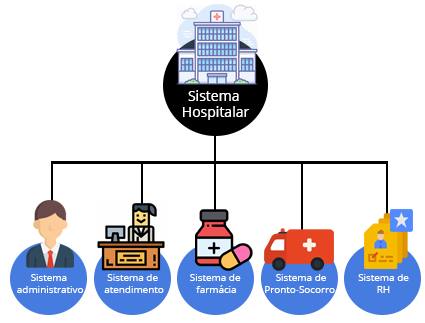
\includegraphics[width=15cm]{DiagramaSubsistema.png} \\

              \end{center}
             \end{figure}
\begin{figure}[H]
              \begin{center}
                  \caption{ Diagrama de redes locais} \label{afp}
                  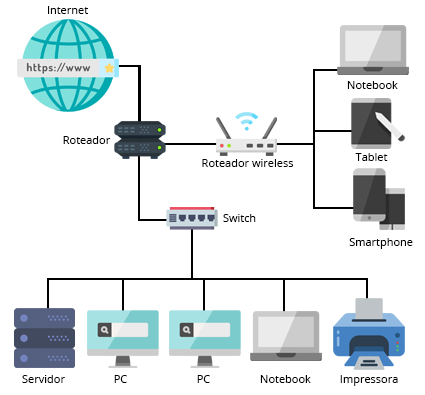
\includegraphics[width=15cm]{DiagramaRede.png} \\

              \end{center}
             \end{figure}

  \subsection{Definição de Requisitos}
1. \textbf{Computadores em todos setores} - Será feita instalação de computadores para sala de consulta, e também para os departamentos de atendimento, administrativo, farmácia, RH e Pronto-Socorro \\\\
3. \textbf{Redes de computadores} - A instalação e manutenção de redes será feita em todos os setores do hospital\\\\
5. \textbf{Equipamento de comunicação entre funcionários} - Todos os funcionários deveram ter um smartphone de uso exclusivo para trabalho\\\\
7. \textbf{Programa de cálculo de rotas para setor Pronto-socor}ro - O sistema de Pronto-socorro deverá ser capaz de calcular melhor rota possível para o atendimento do paciente\\\\
8. \textbf{Programa de gerenciamento de finanças Setor administrativo} - Através do sistema administrativo será possível ter uma visão geral da situação financeira do hospital, além de ser possível gerar relatórios financeiros.\\\\
16. \textbf{Manual do usuári}o - No manual usuário terá todas as informações das funções do sistema.\\\\
18.\textbf{ Catálogos de produtos} - Conterá todos os equipamentos necessários para o funcionamento do sistema\\\\
23.\textbf{ Resultados de exame }- O sistema deverá permitir consultar resultados de exames através de aplicativo, website e diretamente no hospital\\\\
24. \textbf{Controle de estoque de medicamento} - O setor de farmácia terá função de controle de estoque de medicamentos.\\\\
26. \textbf{Treinamento individual para o setor médico e setor de pronto-socorro} - Os treinamentos para setores de RH, administrativo ocorrerão através de uma aula com todos funcionários de determinado setor, os setores de atendimento, Pronto-socorro e o setor médico serão realizado individualmente em um horário de folga.\\\\
27. \textbf{Instalação incremental} - A instalação do sistema será feita aos poucos para não atrapalhar o funcionamento do hospital.\\\\
28. \textbf{Manutenção mensal} - A manutenção do sistema será realizada no final de cada mês para correção de eventuais problemas\\\\
29. \textbf{Backup diário} - Será realizado todos os dias na parte da noite.\\\\
34. \textbf{Aplicativo} - O aplicativo deverá ter a função de marcação de consulta e exames, além de ser possível realizar pagamentos de contas referente ao paciente\\\\
37. \textbf{Pagina web do hospital} - Deverá ter as mesmas funções do aplicativo\\\\
39. \textbf{Dados recentes} - Todos os dados recentes deverão ser feitos backup na nuvem\\


    \subsection{Especificação de requisitos}
2. \textbf{Servidores}\\
2.1 Sala para o servidor\\
2.2 Servidor de Banco de dados\\
2.3 Hospedagem de Website e aplicativo\\
2.4 Servidor de arquivos para compartilhamento de arquivo de um setor para outro\\
2.5 Servidor de e-mail\\
\\
3. \textbf{Redes de computadores}\\
3.1 Compartilhamento de dados\\
3.2 Comunicação entre os funcionários\\
3.3 Internet com Fibra Ótica\\
3.4 Compartilhamento de recursos(impressoras)\\
\\
7. \textbf{Programa de cálculo de rotas para setor Pronto-socorro}\\
7.1 Calculo da distância do trajeto\\
7.2 Previsão de chegada de acordo com a situação do trânsito atual\\
7.3 Permitir ao paciente monitorar em tempo real a chegada do socorro pelo aplicativo/Website\\
7.4 Permitir o desvio de rotas\\
\\
8. \textbf{Programa de gerenciamento de finanças Setor administrativo}\\
8.1 emissão de relatórios\\
8.2 Visão geral das finanças\\
8.3 salvar relatórios\\
8.4 visualizam dos gastos do dia\\
\\
10. \textbf{Sistema de segurança}\\
10.1 Antivírus em todos computadores\\
10.2 Verificação de cadastro usando login\\
10.3 Utilização de CAPTCHA nos login\\
10.4 Autenticação de funcionários será feito por login, senha e biometria\\
\\
24. \textbf{Estoque de medicamento}\\
24.1 Busca pelo medicamento por nome, função do medicamento, laboratório e pelo nome do medico que receitou\\
24.2 Classificação dos medicamentos dever ser feita em ordem alfabética\\
24.3 emitir alertas quando um medicamento está perto da data de validade, e quando já passou da validade\\
24.4 emitir alertas quando um medicamento está com poucas unidades, e quando já acabou um medicamento\\
\\
26. \textbf{Treinamento individual para o setor médico e setor de pronto-socorro}\\
26.1 Aula teórica\\
26.2 Aula Pratica\\
26.3 Prova\\
26.4 Repetição do treinamento em caso de reprovação\\
\\
37. \textbf{Pagina web do hospital}\\
37.1 Opção de marcar/remarca/cancelar de consultas e exames\\
37.2 Visualização de resultados de exames\\
37.3 Realização de pagamentos de contas referente ao paciente, em todas formas de pagamento\\
37.4 Acompanhamento da chegada do socorro em tempo real\\




\section{tipo de requisito}
Nesta secção serão listados os requisitos funcionais, não-funcionais , características não desejáveis, do produto, da organização, da segurança e de negócios.
\subsection{Funcionais}

\begin{enumerate}
  \item Cadastrar produtos para o setor de farmácia
  \item Cadastra pacientes
  \item Gerenciar pacientes
  \item Cadastrar funcionários
  \item Gerenciar funcionários
\end{enumerate}


\subsection{Não funcionais}
\begin{enumerate}
  \item Interface gráfica atrativa
  \item Seguro
  \item Rápido
  \item Fácil na utilização
  \item Funciona em qualquer plataforma
\end{enumerate}


\subsection{Características não desejáveis}

\begin{enumerate}
  \item Lento
  \item Difícil utilização do sistema
  \item Inseguro
  \item Não atender as necessidades dos setores
  \item Interface desorganizada
\end{enumerate}



\subsection{Do Produto}

\begin{enumerate}
  \item Controle de estoque
  \item Redes de internet
  \item Conexão com as redes de impressora
  \item Gerenciamento de serviços
  \item Gerenciamento de RH
\end{enumerate}

\subsection{Da organização}

\begin{enumerate}
  \item Aceitar vários métodos de pagamentos
  \item Medicamento na validade
  \item Garantia dos produtos
  \item Pronto para Reembolso 
  \item Máxima disponibilidade dos meios de comunicação
\end{enumerate}
  

\subsection{Da segurança}

\begin{enumerate}
  \item Acesso
  \item Integridade
  \item Privacidade
  \item Auditoria
  \item Imunidade
\end{enumerate}


\subsection{De negócios}

\begin{enumerate}
  \item Diminuição de desperdícios de medicamento
  \item Diminuição do custo de serviço ao paciente
  \item Diminuição no tempo de processamento
  \item Agilidade no atendimento ao paciente
  \item Fácil cancelamento de consulta/exames
\end{enumerate}

 
  
\section{Stakeholders e Pontos de Vista}

Nesta secção serão apresentados os principais públicos de interesse do sistema os Stakeholders, também será apresentados os pontos de vista do em relação ao projeto.

\subsection{Stakeholders}

\begin{itemize}
  \item Funcionários
  \item Pacientes
  \item Departamento Farmacêutico
  \item Setor Administrativo
  \item Socorristas
  \item Setor de Atendimento
  \item Médicos
  \item Acionistas
  \item Diretor Geral do Hospital
  \item Equipe de manutenção
\end{itemize}
\subsection{ Pontos de vista e serviços}
A seguir será apresentado os pontos de vista, direto e indireto do sistema.
\subsubsection{ Diretos}
\begin{itemize}
  \item \textbf{Pacientes}\\
  -Agendamento de Consultas online\\
-Agendamento de exames online\\
-resultados de exames por aplicativo\\
-Acompanhamento em tempo real do socorro\\
-Pagamento de conta\\

  \item \textbf{Funcionários}\\
 -Ponto pelo sistema\\
-Interface amigável\\
-Emissão de relatórios\\
-Acesso autorizado\\
-Gerenciamento de consultas/exames\\

  \item \textbf{Equipe de manutenção}\\
 -Manutenção de equipamentos\\
-Manutenção de computadores\\
-Manutenção de rede\\
-Instalação de softwares\\
-Instalação de equipamentos\\

  \item \textbf{Equipe do projeto}\\
 -Coleta de Requisitos\\
-Desenvolvimento\\
-Treinamento\\
-Teste com usuários\\
-Implementação\\


  \item \textbf{Engenheiros de rede}\\
-Servidores\\
-Cabeamento de rede\\
-Roteadores wifi\\
-Gerenciamento de rede\\
-Segurança de rede\\

\end{itemize}
\subsubsection{ Indiretos}

\begin{itemize}
  \item \textbf{Setor Administrativo}\\
-Receitas e despesas\\
-Relatórios\\
-Fornecedores\\
-Dividas\\
-Situação financeira\\


  \item \textbf{Direção geral do Hospital}\\
-Gerenciamento de recursos\\
-Relatoria geral\\
-Relatório de todos os setores\\
-Gerenciamento de Funcionários\\
-Contas a pagar\\


  \item \textbf{Fornecedores de medicamentos}\\
-Recebimento de medicamentos\\
-Acesso no Sistema na área de fornecedor\\
-Acompanhamento de medicamento a chegar\\
-Solicitação de medicamento\\
-Relatório de pagamentos\\




  \item \textbf{Acionistas}\\
-Relatórios de ganhos\\
-Situação financeira do Hospital\\
-Informações de todos os setores\\
-Pedido de convocação de reunião\\
-Gerenciamento de reuniões\\



  \item \textbf{Departamento de marketing}\\
-Campanhas\\
-Propagandas Publicitarias\\
-Relatórios das campanhas\\
-Pesquisas de Opinião\\
-Estratégias para atrair pacientes\\
\end{itemize}
\subsection{ Hierarquia de pontos de vista}
Na figura(3.3) está representado os pontos de vista de forma hierárquica de acordo com as prioridades do sistema, e também está organizado em direto e indireto os pontos de vista.
\begin{figure}[H]
              \begin{center}
                  \caption{Hierarquia de pontos de vista} \label{afp}
                  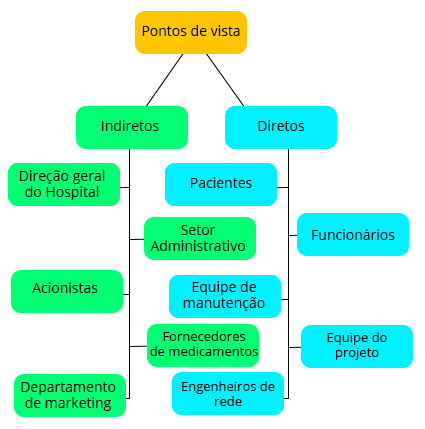
\includegraphics[width=15cm]{HierarquiaPontoVista.png} \\

              \end{center}
             \end{figure}

\section{Entrevista}
A entrevista é uma técnica importante e a mais usada forma de coleta de requisitos para um sistema.  Foram selecionadas 8 perguntas que serão realizadas, para o entendimento do sistema antigo e para possíveis melhorias para o novo sistema. A entrevista será feita com um funcionário no cargo de atendente do setor de atendimento. Foi escolhido o funcionário do setor de atendimento pelo motivo de ser o setor que mais utiliza o sistema. \\

\begin{enumerate}
  \item \textbf{O que você acha do sistema atual?}
  \\R:Eu acho que é um sistema ultrapassado, pois não encaixa no mundo em que vivemos atualmente. O sistema não oferece nenhum tipo de facilidade para os funcionários e para os pacientes, e isso acaba dificultando atrair novos pacientes e no atendimento dos mesmos \\

  \item \textbf{No sistema de qual forma os pacientes marcam consultas/exames? Qual sua opinião sobre?}
  \\R:Eu acho que é um sistema ultrapassado, pois não encaixa no mundo em que vivemos atualmente. O sistema não oferece nenhum tipo de facilidade para os funcionários e para os pacientes, e isso acaba dificultando atrair novos pacientes e no atendimento dos mesmos \\

  \item \textbf{Quais são alguns dos problemas que você enfrenta diariamente?}
  \\R: A única forma de marca consulta e exames, como disse anteriormente, e as poucas funções que o sistema oferece, que acaba limitando o atendimento ao paciente. Como por exemplo: No sistema não existi a função de realizar pagamentos via cartão, e uma outra função que não tem, é a diversidade de formas para o paciente pegar resultados de exames, pois atualmente a única forma de pegar o resultado é diretamente aqui no hospital. \\

  \item \textbf{Quais são melhorias que você gostaria de ver?}
  \\R:Diversidade na forma de marca consultas e exames, como dito anteriormente acaba criando filas. Outras melhorias seria mais opção de formas de pagamentos e outros meios do paciente receber os resultados de exames \\

  \item \textbf{O que você acha da interface do sistema atual?}
  \\R:Não acho intuitiva, pois a interface do sistema funciona por linhas de comandos, e isso acaba dificultando no entendimento do sistema para os novos funcionários. \\

  \item \textbf{O sistema atual é fácil de operar ?}
  \\R:Não, como dito anteriormente o sistema funciona por linhas de comandos, complicando assim de usar o sistema pois tem que ficar decorando comando para realizar as funções. \\

  \item \textbf{Você utiliza todas as funções do sistema atual?}
  \\R:Não, existir algumas na qual não tenho conhecimento de sua funcionalidade, pois no treinamento não foi mencionado da serventia dessas funções. \\

  \item \textbf{O que você adicionaria no novo sistema?}
  \\R:Adicionaria a opção de marca ponto através do próprio sistema, essa opção irar diminuir a perda de tempo ao se deslocar para o local que marca o ponto dos funcionários, quando um funcionário logar no sistema automaticamente será marcado o ponto.
\end{enumerate}

\subsection{Relatório da entrevista}
    
Através da entrevista, pode percebe-se que o sistema atual é ultrapassado e não atende as necessidades dos funcionários e dos pacientes. Os principais problemas observados foram a falta de diversidades nas formas de pagamento, falta de meios na marcação de consultas e exames, e a visualização de resultados de exames. Foi notado também a falta de intuitividade da interface, que no sistema atual funciona através de linhas de comandos dificultando a adaptação de novos funcionários.
    
Foi observado também que os funcionários não tem o conhecimento das funcionalidades de algumas funções do sistema, proporcionando assim a não utilização de algumas funções. Isso se deve ao fato do péssimo treinamento dos funcionários em relação ao sistema. Foi sugerido pelo funcionário entrevistado a marcação de ponto pelo sistema, com o objetivo de diminuir o tempo de deslocamento dos funcionários ao local de bater o ponto.




\section{ Casos de Uso}
Nesta secção serão apresentados os casos de uso do sistema, que tem como finalidade representar as interações realizadas pelo usuário e as respostas do sistema.
    \subsection{ Cadastro de paciente}
\begin{enumerate}
  \item Login no sistema
  \item Preenchimento dos dados do paciente
  \item Verificação de dados já existente
  \item Confirmação dos dados
  \item Escolha do método de pagamento
  \item Gerar ID do paciente
  \item Finalizar cadastro
  \item Gerar relatório
\end{enumerate}

    \subsection{ Cadastro de medicamento no setor farmacêutico}
\begin{enumerate}
  \item Login no sistema
  \item Preenchimento de dados do medicamento
  \item Informar valor pago pelo medicamento
  \item Atualizar estoque de medicamento
  \item Finalizar cadastro
  \item Gerar relatório
\end{enumerate}


    \subsection{ Cadastro de funcionário no setor RH}
\begin{enumerate}
  \item Login no sistema
  \item Preenchimento de dados pessoais do funcionário
  \item Informa o setor
  \item Informa o cargo
  \item Calcular salário inicial
  \item Preencher informações de pagamento de salário
  \item Gerar ID do funcionário
  \item Finalizar cadastro
  \item Gerar relatório

\end{enumerate}

    \subsection{ Diagrama de caso de uso}
    O diagrama a seguir tem como finalidade mostrar graficamente o caso de um “atendimento ao um paciente”.
    \begin{figure}[H]
              \begin{center}
                  \caption{ Diagrama de caso de uso de atendimento ao um paciente} \label{afp}
                  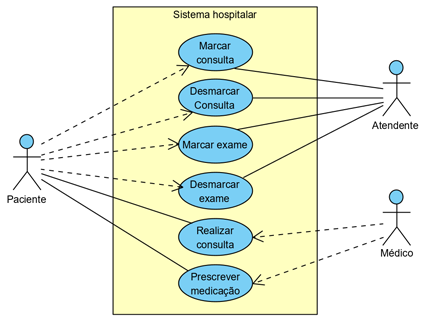
\includegraphics[width=15cm]{CasoDeUso.png} \\

              \end{center}
             \end{figure}




    \subsection{ Diagrama de caso de uso}
    Tem como objetivo representar graficamente o caso de uso do sistema além de mostrar informações do mesmo.
\section{ Diagramas de fluxo de dados}
É uma forma de representar graficamente os relacionamentos entre processos com as bases de dados do sistema.

    \subsection{Diagrama de contexto}
    Tem como objetivo permitir ter um panorama geral de todo sistema. Com o objetivo geral do sistema.
    \begin{figure}[H]
              \begin{center}
                  \caption{ Diagrama de contexto} \label{afp}
                  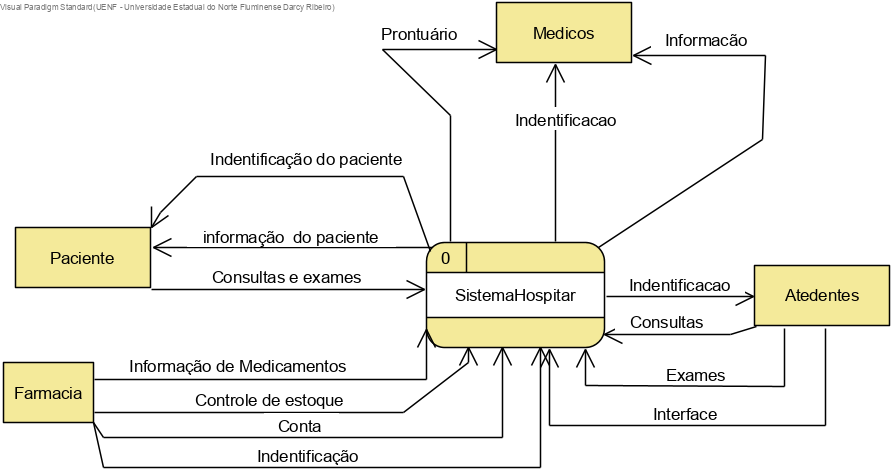
\includegraphics[width=15cm]{1.png} \\

              \end{center}
             \end{figure}

    \subsection{Diagrama do sistema }
    O diagrama do sistema tem como finalidade mostrar o sistema completo, com todos os fluxos de dados e divisões do sistema.

     \begin{figure}[H]
              \begin{center}
                  \caption{Diagrama do sistema} \label{afp}
                  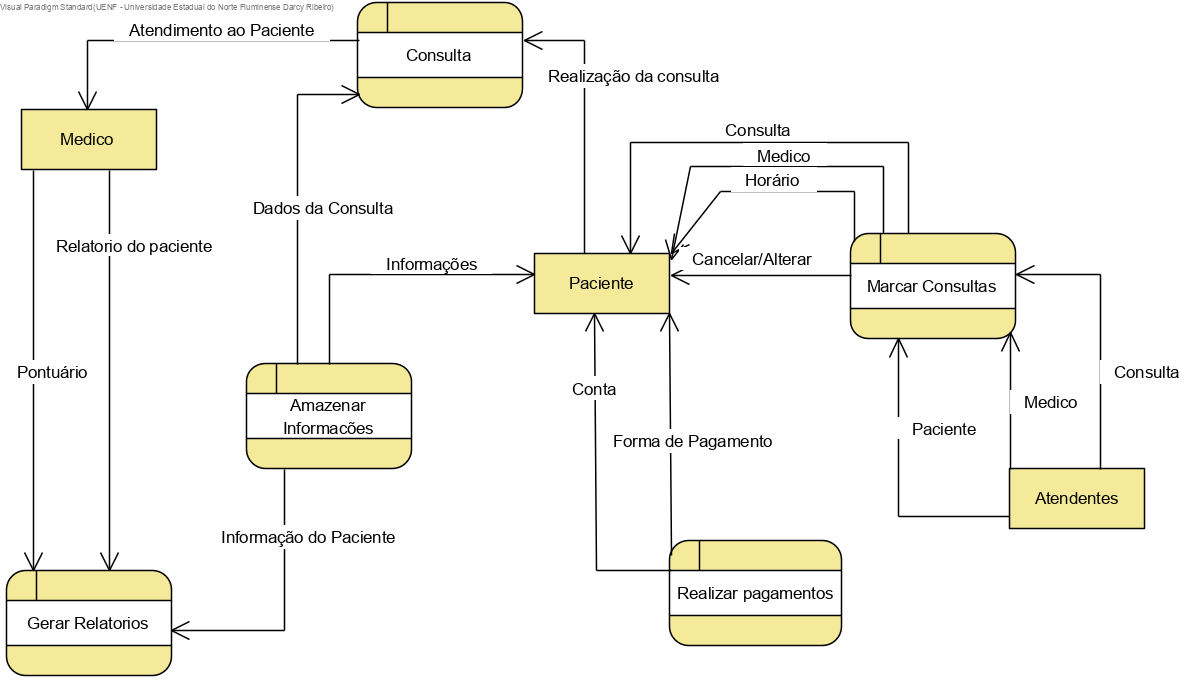
\includegraphics[width=15cm]{2.png} \\

              \end{center}
             \end{figure}


             \begin{figure}[H]
              \begin{center}
                  \caption{Diagrama do sistema nivel 1} \label{afp}
                  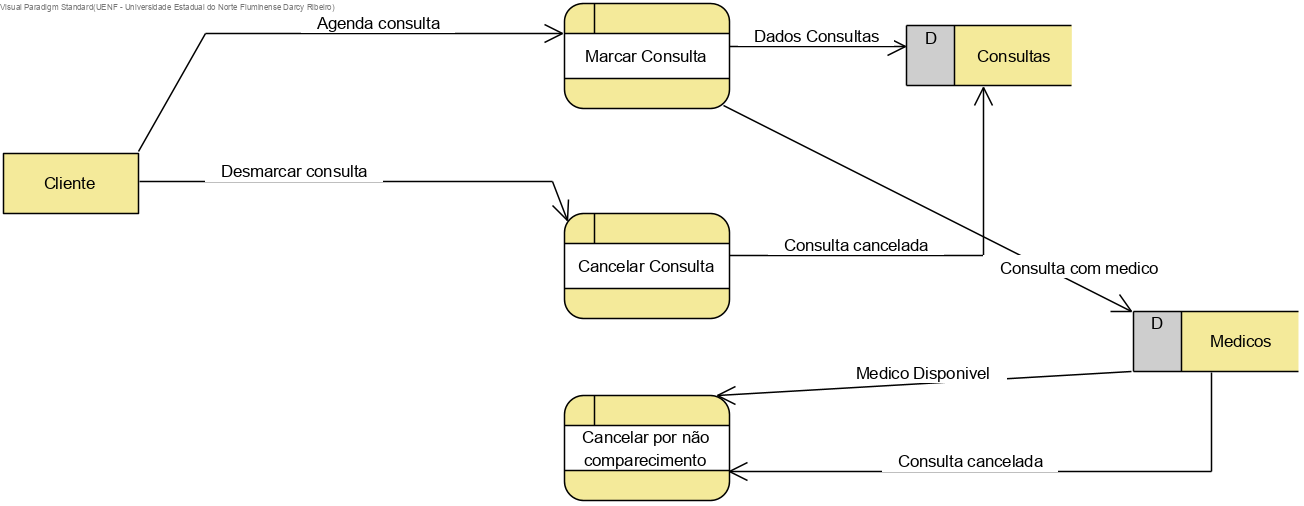
\includegraphics[width=15cm]{3.png} \\

              \end{center}
             \end{figure}

\section{ Diagramas de entidades e relacionamentos}

A secção a seguir mostra os diagramas que tem como finalidade realizar a modelagem do relacionamento entre as entidades. Serão representados 4 diagramas de relacionamento, subsistema de farmácia(3.8 ), atendimento presencial ao paciente(3.9),  subsistema de RH(3.10) e paciente no aplicativo (3.11) .
              \begin{figure}[H]
              \begin{center}
                  \caption{Subsistema de farmácia} \label{afp}
                  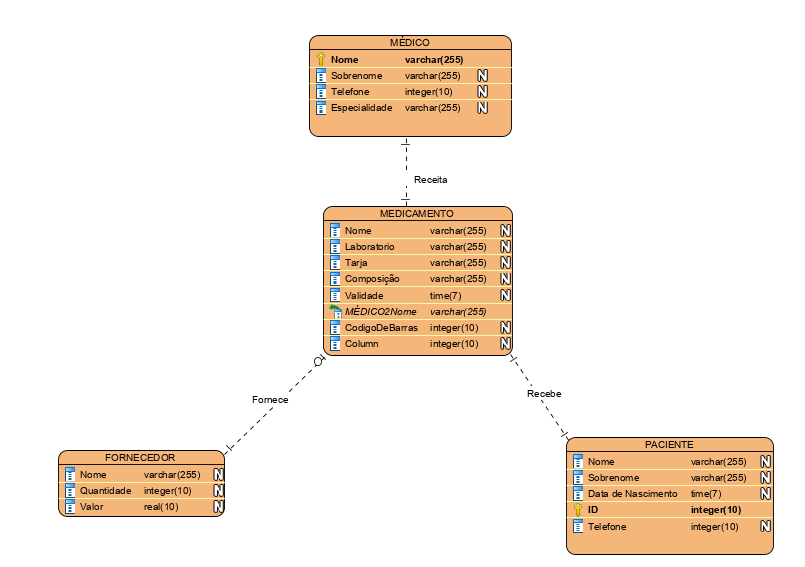
\includegraphics[width=15cm]{SubsistemaDeFarmacia.png} \\

              \end{center}
             \end{figure}
             
             
                      \begin{figure}[H]
              \begin{center}
                  \caption{Atendimento presencial ao paciente} \label{afp}
                  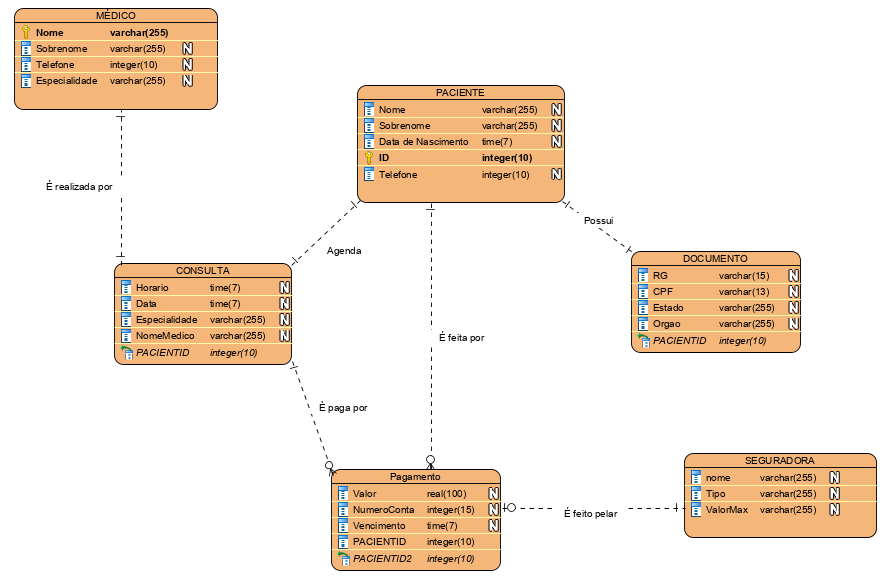
\includegraphics[width=12cm]{AtendimentoPresencialAoPaciente.png} \\

              \end{center}
             \end{figure}
             
                    \begin{figure}[H]
              \begin{center}
                  \caption{Subsistema de RH} \label{afp}
                  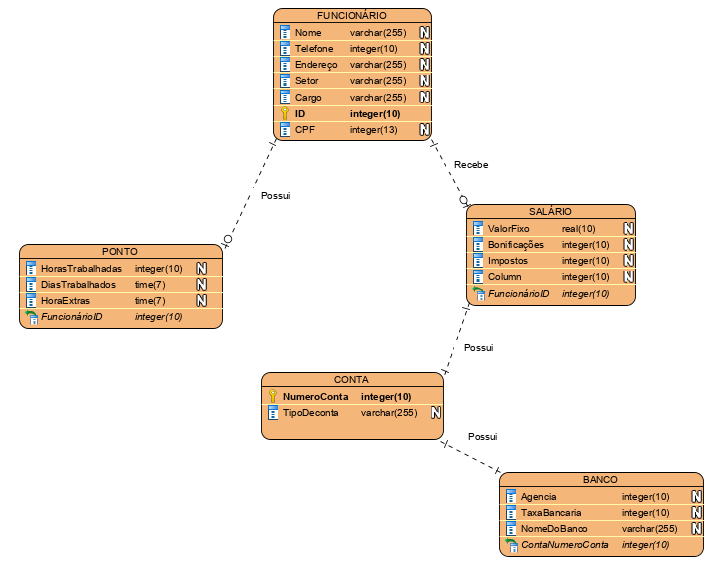
\includegraphics[width=15cm]{SubsistemaDeRH.png} \\

              \end{center}
             \end{figure} 

              \begin{figure}[H]
              \begin{center}
                  \caption{Paciente no aplicativo } \label{afp}
                  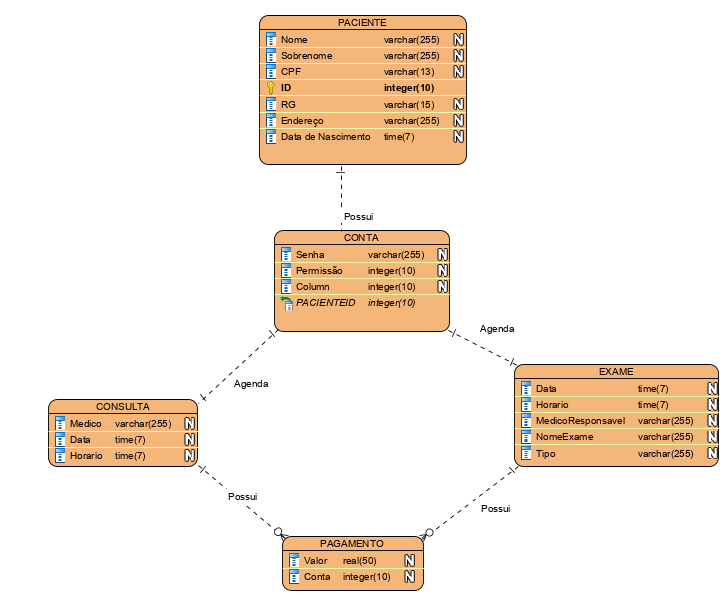
\includegraphics[width=15cm]{PacienteNoAplicativo.png} \\
              \end{center}
             \end{figure}
     






         